% Copyright (c)  2010-2011  EADS.
% Permission is granted to copy, distribute and/or modify this document
% under the terms of the GNU Free Documentation License, Version 1.2
% or any later version published by the Free Software Foundation;
% with no Invariant Sections, no Front-Cover Texts, and no Back-Cover
% Texts.  A copy of the license is included in the section entitled "GNU
% Free Documentation License".




%%%%%%%%%%%%%%%%%%%%%%%%%%%%%%%%%%%%%%%%%%%%%%%%%%%%%%%%%%%%%%%%%%%%%%%%%%%%%%%%%%%%%%%%%% 
\section{Use Cases Guide}

This section presents the main functionalities of the module $otmixmod$ in their context.



%%%%%%%%%%%%%%%%%%%%%%%%%%%%%%%%%%%%%%%%%%%%%%%%%%%%%%%%%%%%%%
\subsection{Which python modules to import ?}

In order to use the functionalities described in this documentation, it is necessary to import  : 
\begin{itemize}
   \item the $openturns$ python module which gives access to the Open TURNS functionalities,
   \item the $otmixmod$ module which links the $openturns$ functionalities and MIXMOD .
\end{itemize}

Python  script for this use case :

\begin{lstlisting}
# Load OpenTURNS to manipulate distributions
from openturns import *
# Load the link between OT and MIXMOD
from otmixmod import *
\end{lstlisting}

\subsection{Creation of a Factory} \label{FactoryCreation}

In $otmixmod$, it is possible to create a factory for the mixture distribution. The parameters are:
\begin{itemize}
 \item the number of atoms (mandatory argument),
 \item the covariance model (optional argument), $CovarianceModel$.
\end{itemize}

We will apply it to a $NumericalSample$ to get the mixture.

\subsubsection{UC : Creation of a Covariance Model (optional)}

A Covariance Model is the covariance model assumed for the several atoms of a mixture. \\

\requirements{
  \begin{description}
  \item[$\bullet$] none
  \end{description}
}
{
  \begin{description}
  \item[$\bullet$] a CovarianceModel variable  : {\itshape myCovarianceModel},
  \item[type:] a CovarianceModel
  \end{description}
}
\espace

Many covariance models are implemented in MIXMOD. The covariance models that are available are listed in tab \ref{tab:listCovarianceModels} (cf. MIDMOD documentation for their meaning).


\begin{table}
\centering
 \begin{tabular}{|l|l|}\hline
Model   &   Categories  \\\hline
Gaussian\_p\_L\_I   &  Spherical\\ 
Gaussian\_p\_Lk\_I   &    \\ \hline
Gaussian\_p\_L\_B   &  Diagonal\\
Gaussian\_p\_Lk\_B   &    \\
Gaussian\_p\_L\_Bk   &    \\
Gaussian\_p\_Lk\_Bk   &    \\\hline
Gaussian\_p\_L\_C   &   General \\
Gaussian\_p\_Lk\_C   &    \\
Gaussian\_p\_L\_D\_Ak\_D   &    \\
Gaussian\_p\_Lk D\_Ak\_D   &    \\
Gaussian\_p\_L\_Dk\_A\_Dk   &    \\
Gaussian\_p\_Lk\_Dk\_A\_Dk   &    \\
Gaussian\_p\_L\_Ck   &    \\
Gaussian\_p\_Lk\_Ck   &    \\\hline
Gaussian\_pk\_L\_I   &  Spherical\\ 
Gaussian\_pk\_Lk\_I   &    \\ \hline
Gaussian\_pk\_L\_B   &  Diagonal\\
Gaussian\_pk\_Lk\_B   &    \\
Gaussian\_pk\_L\_Bk   &    \\
Gaussian\_pk\_Lk\_Bk   &    \\\hline
Gaussian\_pk\_L\_C   &   General \\
Gaussian\_pk\_Lk\_C   &    \\
Gaussian\_pk\_L\_D\_Ak\_D   &    \\
Gaussian\_pk\_Lk D\_Ak\_D   &    \\
Gaussian\_pk\_L\_Dk\_A\_Dk   &    \\
Gaussian\_pk\_Lk\_Dk\_A\_Dk   &    \\
Gaussian\_pk\_L\_Ck   &    \\
Gaussian\_pk\_Lk\_Ck   &    \\\hline
\end{tabular}
\caption{The 28 Gaussian Models (Covariance Structure) \label{tab:listCovarianceModels}}
\end{table}

\espace
Python script for this use case:

\begin{lstlisting}
 # Create a CovarianceModel
myCovModel = Gaussian_pk_Lk_C()
\end{lstlisting}


\subsection{Creation of a Factory} %\label{FactoryCreation}

The mixture factory is built from the number of atoms and the covariance model.

\requirements{
  \begin{description}
  \item[$\bullet$] the atoms number : {\itshape atomsNumber},
  \item[type:] UnsignedInteger
  \item[$\bullet$] a CovarianceModel variable, optional: {\itshape myCovarianceModel} (default value $Gaussian\_pk\_Lk\_C$)
  \item[type:] CovarianceModel
  \end{description}
}
{
  \begin{description}
  \item[$\bullet$] a Mixture factory: {\itshape myMixtureFactory},
  \item[type:] MixtureFactory
  \end{description}
}

\espace
Python script for this use case:

\begin{lstlisting}
atomsNumber = 3
factory = MixtureFactory(atomsNumber, myCovModel)
\end{lstlisting}

\subsection{Estimation of the Mixture parameters}

It is now possible to estimate the mixture parameters from a numerical sample.

\requirements{
  \begin{description}
  \item[$\bullet$] a Mixture factory : {\itshape myMixtureFactory},
  \item[type:] MixtureFactory
  \item[$\bullet$] a numerical sample : {\itshape mySample},
  \item[type:] NumericalSample
  \end{description}
}
{
  \begin{description}
  \item[$\bullet$] a Mixture distribution : {\itshape myEstimatedMixture},
  \item[type:] Distribution
  \end{description}
}
\espace

\espace
Python script for this use case:

\begin{lstlisting}
# Estimate the mixture parameters
# We estimate all the parameters of the Mixture distribution from sample
estimatedDistribution = factory.build(sample)

# Display the resulted distribution with its parameters
print "Estimated distribution=", estimatedDistribution

# If the sample has a dimension 2, we draw the estimated pdf and the sample
if sample.getDimension() == 2 : 
    g = estimatedDistribution.drawPDF()
    c = Cloud(sample)
    c.setColor("red")
    c.setPointStyle("bullet")
    ctmp = g.getDrawable(0)
    g.setDrawable(Drawable(c), 0)
    g.addDrawable(ctmp)
    g.draw("testMixtureEstimation")

\end{lstlisting}
The estimated distribution can be manipulated as a classical mixture distribution. So, in the case of a 1D- or 2D-sample it is possible to draw the estimated pdf and the sample on the same graph, cf. figure \ref{fig:showMixmodResult}.

\begin{figure}[h]
 \centering
 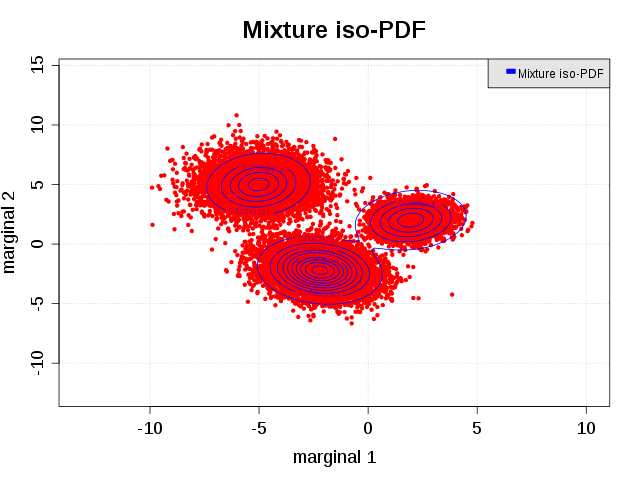
\includegraphics[scale=0.4]{testMixMod.png}
 % testMixMod.png: 640x480 pixel, 72dpi, 22.58x16.94 cm, bb=0 0 640 480
 \caption{Estimated mixture and Numerical Sample}
 \label{fig:showMixmodResult}
\end{figure}

\subsection{Estimation of the Mixture parameters and classification}

It is now possible to estimate the mixture parameters from a numerical sample and to classify its points.

\requirements{
  \begin{description}
  \item[$\bullet$] a Mixture factory : {\itshape myMixtureFactory},
  \item[type:] MixtureFactory
  \item[$\bullet$] a numerical sample : {\itshape mySample},
  \item[type:] NumericalSample
  \end{description}
}
{
  \begin{description}
  \item[$\bullet$] a Mixture distribution : {\itshape myEstimatedMixture},
  \item[type:] Distribution
  \item[$\bullet$] an Indices : {\itshape labels},
  \item[type:] Indices
  \item[$\bullet$] a NumericalPoint : {\itshape BICLogLikelihood},
  \item[type:] NumericalPoint
  \end{description}
}
\espace

\espace
Python script for this use case:

\begin{lstlisting}
# Estimate the mixture parameters
# We estimate all the parameters of the Mixture distribution from a sample,
# the labels of the points in the sample and the corresponding BIC Log Likelihood

bestLogLikelihood = -1e100
bestNbClusters = 0
bestLabels = Indices(0)
for nbClusters in range(1, 11):
    factory = MixtureFactory(nbClusters)
    labels = Indices(0)
    logLikelihood = NumericalPoint(0)
    estimatedDistribution = factory.build(sample, labels, logLikelihood)
    # Only the second component (i.e with index 1) is usefull for selection purpose
    if logLikelihood[1] > bestLogLikelihood:
        bestLogLikelihood = logLikelihood[1]
        bestNbClusters = nbClusters
        bestLabels = labels
print "best nb clusters=", bestNbClusters, "BIC log-likelihood=", bestLogLikelihood

# Classify the points
partition = list(NumericalSample(0, sample.getDimension()) for i in range(bestNbClusters))
for i in range(sample.getSize()):
    partition[labels[i]].add(sample[i])
# Print the partition
for i in range(bestNbClusters):
    print "cluster", i, "=", partition[i]
\end{lstlisting}
The partitioning can be used to build local meta-models for example, in a mixture of experts approach.